\begin{frame}[t]{Transport-Corrected Scattering Approximation}
    
    \begin{itemize}
        \item Modifies self-scatter and total cross-sections to account for 
        anisotropy while performing isotropic calculations
        \item Neutron Leakage Conservation (NLC) Method: H-1
        \begin{equation*}
        \Sigma_{s0,g\rightarrow g} = \Sigma_{s0,g\rightarrow g} + \frac{1}{3D_g} 
        - \Sigma_{t,g}
        \end{equation*}
        \item In-Scatter Method: B-11, C-12, O-16
        \begin{equation*}
        \Sigma_{s0,g\rightarrow g} = \Sigma_{s0,g\rightarrow g} - 
        \frac{1}{\phi_{1,g}}\sum_{g'=1}^G \Sigma_{s1,g'\rightarrow g}\phi_{1,g'}
        \end{equation*}
        \item Out-Scatter Method: All other isotopes
        \begin{equation*}
        \Sigma_{s0,g\rightarrow g} = \Sigma_{s0,g\rightarrow g} - \sum_{g'=1}^G 
        \Sigma_{s1,g\rightarrow g'}
        \end{equation*}
    \end{itemize}
    
\end{frame}

%%%%%%%%%%%%%%%%%%%%%%%%%%%%%%%%%%%%%%%%%%%%%%%%%%%%%%%%%%%%%%%%%%%%%%%%%%%%%%%%%

\begin{frame}[t]{2D MOC}
    
    \begin{columns}
        \begin{column}{0.6\textwidth}
            \begin{itemize}
                \item Solve along a specific direction $\Omega_n$
                \begin{equation*}\scriptstyle
                \bm r = \bm {r_0} + s \bm \Omega_n \Rightarrow \begin{cases} 
                x\left(s\right) = x_0 + s\Omega_{n,x} \\ y\left(s\right) = y_0 + 
                s\Omega_{n,y} \\ z\left(s\right) = z_0 + s\Omega_{n,z} \end{cases}
                \end{equation*}
                \item Problem reduces from PDE to ODE that can be solved analytically
                \begin{equation*}\scriptstyle
                \frac{\partial \psi_{g,n}}{\partial s} + \Sigma_{t,g}\left(\bm r_0 + 
                s\bm\Omega_n\right)\psi_{g,n}\left(\bm r_0 + s\bm\Omega_n\right) = 
                q_{g,n}\left(\bm r_0 + s\bm\Omega_n\right)
                \end{equation*}
                \begin{dmath*}\scriptstyle
                    {\psi_{g,n}\left(\bm r_0 + s\bm\Omega_n\right) = \psi_{g,n}\left(\bm 
                        r_0\right)\exp{\left(-\intop_0^s \Sigma_{t,g}\left(\bm r_0 + 
                            s'\bm\Omega_n\right)ds'\right)}} + {\intop_0^s q_{g,n}\left(\bm r_0 + 
                        s'\bm\Omega_n\right)\exp{\left(-\intop_0^{s'} \Sigma_{t,g}\left(\bm r_0 
                            + s''\bm\Omega_n\right)ds''\right)}ds'}
                \end{dmath*}
            \end{itemize}
        \end{column}
        \begin{column}{0.4\textwidth}
            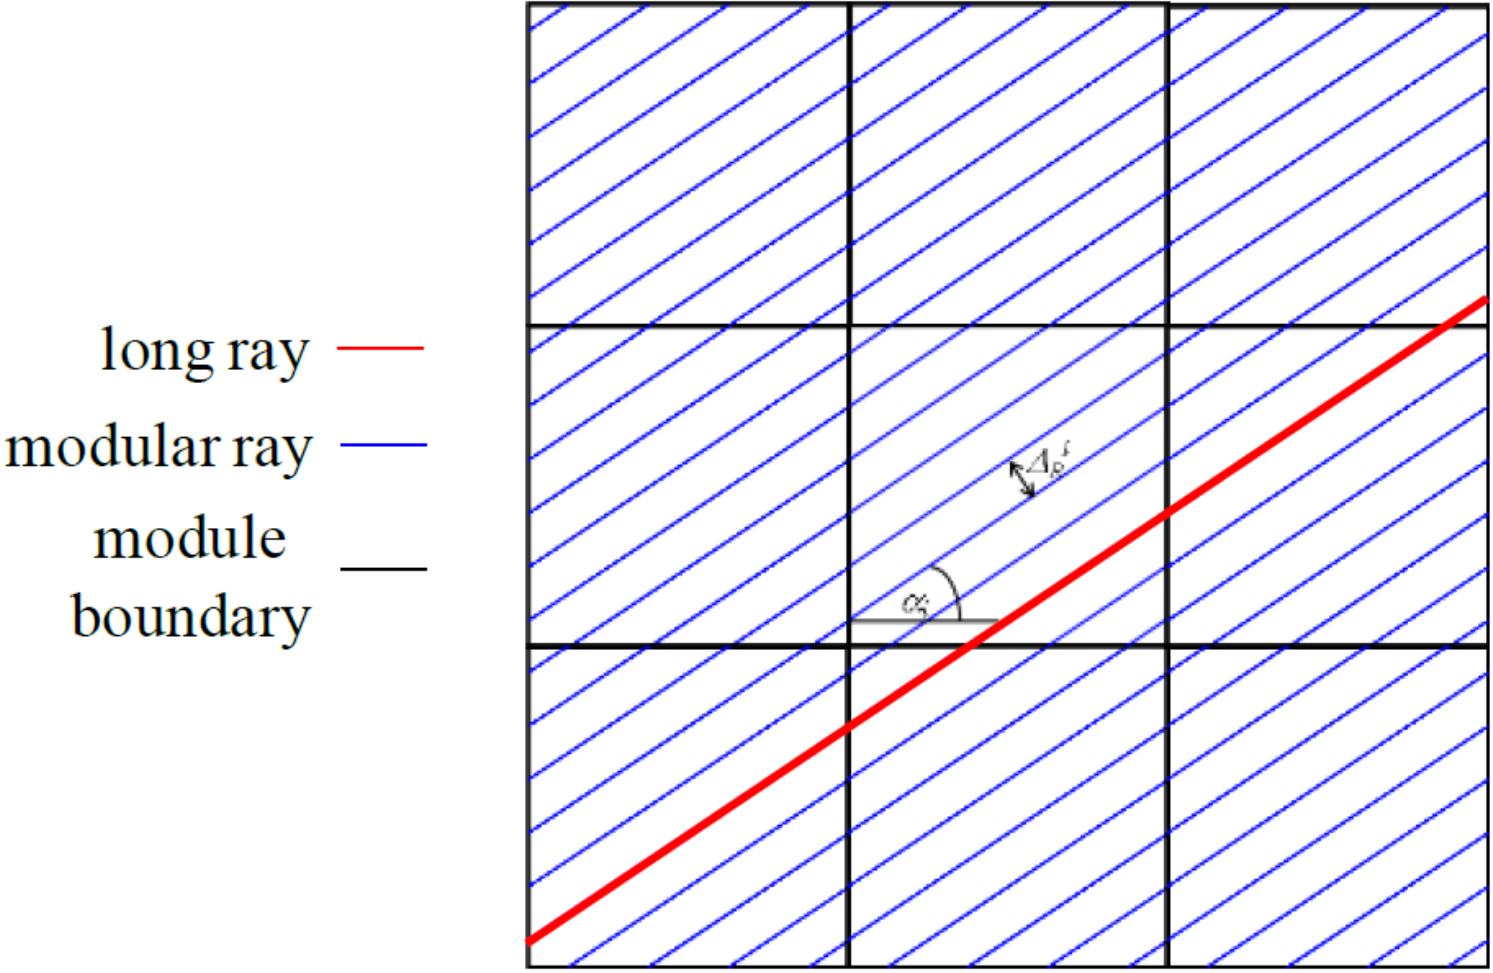
\includegraphics[width=\textwidth]{modular_rays.png}
        \end{column}
    \end{columns}
    
\end{frame} 

%%%%%%%%%%%%%%%%%%%%%%%%%%%%%%%%%%%%%%%%%%%%%%%%%%%%%%%%%%%%%%%%%%%%%%%%%%%%%%%%%

\begin{frame}[t]{2D MOC}
    
    \begin{itemize}
        \item Assume flat source, cross-section along track with 
        length $L_j$ and spacing $\delta x$
        \begin{columns}
            \begin{column}{0.6\textwidth}
                \begin{align*}\scriptstyle
                \psi^{out}_{g,i,n,j} &\scriptstyle = \psi^{in}_{g,i,n,j}e^{-\Sigma_{t,g,i} 
                    L_j} 
                \\\scriptstyle
                &\scriptstyle + \frac{q_{g,i,n}}{\Sigma_{t,g,i}}\left(1 - 
                e^{-\Sigma_{t,g,i}L_j}\right) \\\scriptstyle
                \overline{\psi}_{g,i,n,j} &\scriptstyle = 
                \frac{q_{g,n,i}}{\Sigma_{t,g,i}} 
                \\\scriptstyle
                &\scriptstyle + \frac{1 - e^{-\Sigma_{t,g,i} 
                        L_j}}{L_j\Sigma_{t,g,i}}\left(\psi^{in}_{g,i,n,j} - 
                \frac{q_{g,n,i}}{\Sigma_{t,g,i}}\right) \\\scriptstyle
                \overline{\psi}_{g,i,n} &\scriptstyle = \frac{\sum_j 
                    \overline{\psi}_{g,i,n,j} \delta x L_j}{\sum_j \delta x L_j}
                \end{align*}
            \end{column}
            \begin{column}{0.4\textwidth}
                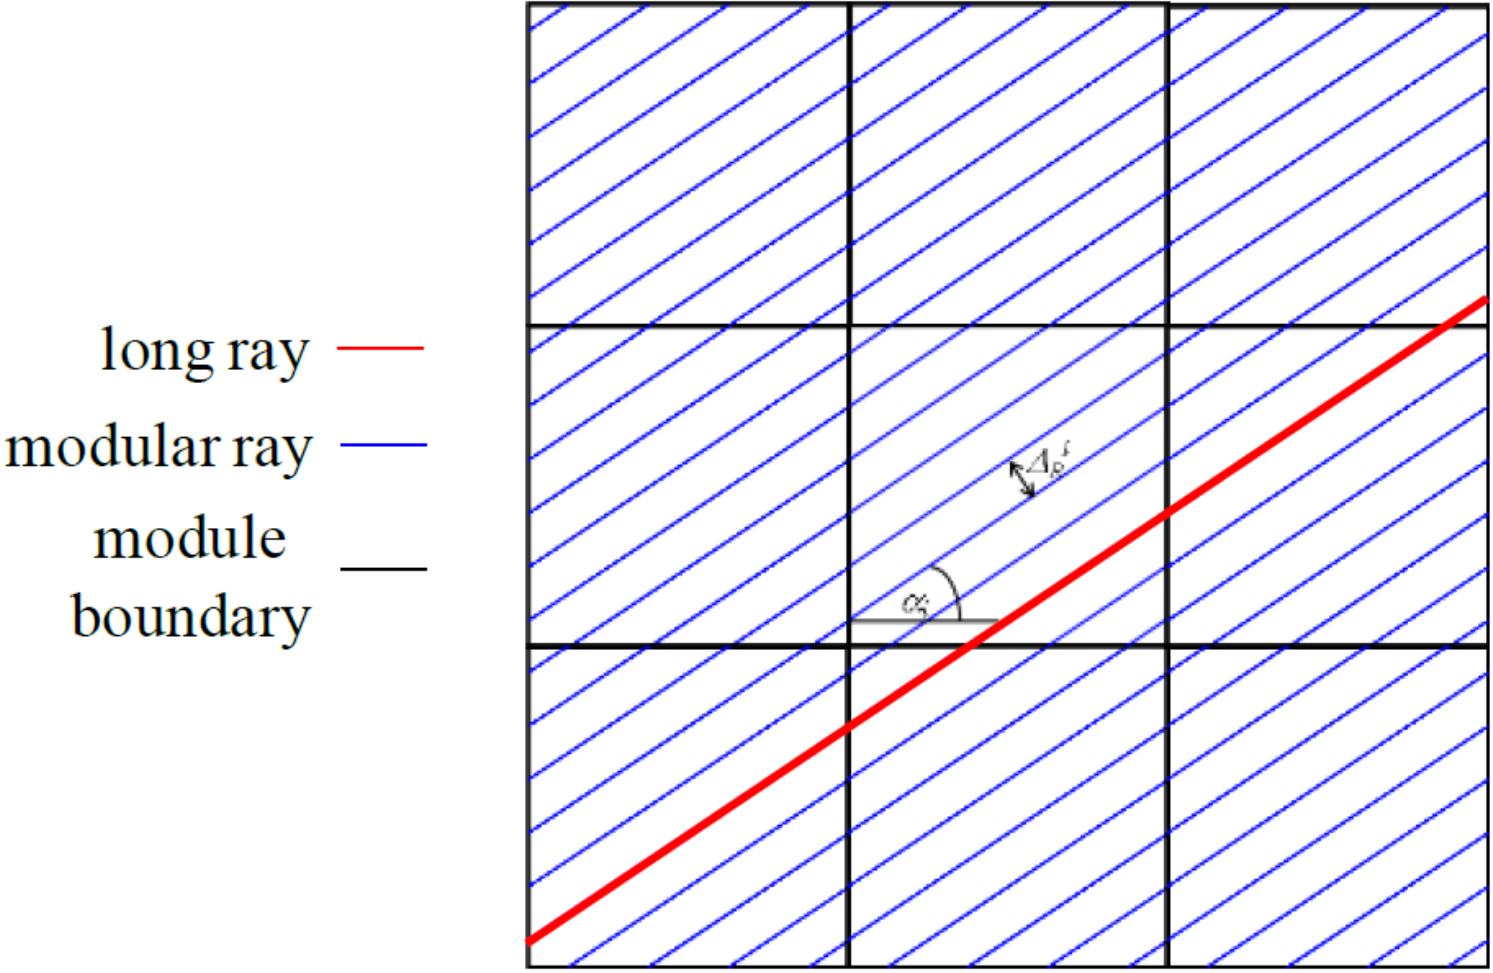
\includegraphics[width=\textwidth]{modular_rays.png}
            \end{column}
        \end{columns}
        \item Modular ray tracing can be used to minimize storage requirements by 
        tracing only portions of problem geometry
    \end{itemize}
    
\end{frame} 

%%%%%%%%%%%%%%%%%%%%%%%%%%%%%%%%%%%%%%%%%%%%%%%%%%%%%%%%%%%%%%%%%%%%%%%%%%%%%%%%%

\begin{frame}[t]{2D MOC}
    
    \begin{columns}
        \begin{column}{0.55\textwidth}
            \begin{itemize}
                \item Perform ray tracing and store segment information up front
                \item Set up scattering, fission, and axial transverse leakage sources
                \begin{itemize}
                    \item Multi-group sweeping
                    \item 1-group sweeping
                \end{itemize}
                \item Parallel Decomposition
                \begin{itemize}
                    \item Spatial (Planar and Radial)- MPI
                    \item Angle - MPI
                    \item Ray - OpenMP
                \end{itemize}
            \end{itemize}
        \end{column}
        \begin{column}{0.45\textwidth}
            \begin{figure}[h]
                \centering
                \resizebox{!}{0.7\textheight}{\begin{tikzpicture}[node distance=2cm]

% Begin
\node (start) [startstop] {Start};
\node (init) [io, right of=start, xshift=2.5cm] {Input N$_{inners}$};

% MOC
\node (begin) [process, below of=init] {Set $n=0$};
\node (source) [process, below of=begin] {Calculate fission and axial transverse leakage sources};
\node (scatSource) [process, below of=source] {Calculate scattering source};
\node (MOC) [process, below of=scatSource] {2D MOC sweep over each energy group};
\node (MOCdone) [decision, below of=MOC, yshift=-1.5cm] {$n = N_{inners}$?};z
\node (stop) [startstop, right of=MOCdone, xshift=2.5cm] {Stop};

% Basic Arrows
\draw [arrow] (start) -- (init);
\draw [arrow] (init) -- (begin);
\draw [arrow] (begin) -- (source);
\draw [arrow] (source) -- (scatSource);
\draw [arrow] (scatSource) -- (MOC);
\draw [arrow] (MOC) -- (MOCdone);

% Fancy Arrows
\draw [arrow] (MOCdone) -| node[anchor=north] {no} ([xshift=-1.5cm]MOC.west) |- (scatSource);
\draw [arrow] (MOCdone) -- node[anchor=north] {yes} (stop);

\end{tikzpicture}}
            \end{figure}
        \end{column}
    \end{columns}
    
\end{frame}

%%%%%%%%%%%%%%%%%%%%%%%%%%%%%%%%%%%%%%%%%%%%%%%%%%%%%%%%%%%%%%%%%%%%%%%%%%%%%%%%%